% !TeX root = ../DoABook.tex
\chapter{مقدمه}
\label{chap:introduction}

کاربردهای فناوری‌های بی‌سیم در حوزه‌های گوناگونی گسترش یافته‌اند؛ از جمله پایش محیط‌زیست، شبکه‌های حسگر، امنیت عمومی و عملیات جست‌وجو و نجات. در پرتو این تحولات، سیاست‌ها و مقررات فناورانه متعددی برای پاسخ‌گویی به نیازهای مختلف تدوین شده‌اند. برای مثال، کمیسیون ارتباطات فدرال\LTRfootnote{Federal Communications Commission} در یک مقررات الزامی اعلام کرده است که دقت مکان‌یابی تماس‌های اضطراری بی‌سیم باید به $125$ متر برسد~\cite{1}. همچنین در عملیات جست‌وجو و نجات معمولاً تعیین مکان منابع بیکن الکترومغناطیسی ضروری است. همه این کاربردها را می‌توان از دلایل اصلی افزایش توجه اخیر به تعیین \textit{جهت ورود سیگنال‌های رادیویی}\LTRfootnote{Direction of Arrival} در سامانه‌های بی‌سیم دانست. در واقع، تخمین جهت ورود چندین سیگنال رادیویی که به یک آرایه از حسگرها برخورد می‌کنند، در بسیاری از کاربردهای دیگر نیز مورد نیاز است؛ از جمله رادار، سونار و لرزه‌شناسی. فناوری دیگری که در سال‌های اخیر توجه زیادی را به خود جلب کرده است، \textit{فناوری آنتن هوشمند}\LTRfootnote{Smart Antenna Technology} است~\cite{2,3}. در این فناوری معمولاً یک الگوریتم تخمین جهت ورود سیگنال به‌کار گرفته می‌شود تا سامانه‌هایی توسعه یابند که اطلاعات مکان‌یابی دقیقی برای خدمات بی‌سیم فراهم کنند~\cite{4}.

در چارچوب مباحث این کتاب، \textit{آنتن هوشمند} سامانه‌ای است که چندین المان آنتنی را با قابلیت پردازش سیگنال ترکیب می‌کند تا الگوی تابش و/یا دریافت خود را به‌صورت خودکار و متناسب با محیط سیگنالی سامانه بهینه کند. این فناوری به‌ویژه در ارتباطات سیار، با توجه به افزایش تعداد مشترکان و محدود بودن منابع، بسیار مفید واقع شده است. آنتن‌های هوشمند می‌توانند از طریق افزایش برد پوشش، محدوده سرویس‌دهی را گسترش دهند و همچنین ظرفیت سامانه را افزایش دهند~\cite{2,3}.

آنتن‌های هوشمند همچنین قادرند سیگنال‌ها را از نظر مکانی از یکدیگر جدا کنند؛ به‌گونه‌ای که مشترکان مختلف بتوانند از منابع طیفی یکسان استفاده کنند، مشروط بر آنکه در ایستگاه پایه از نظر مکانی قابل تفکیک باشند. این روش که \textit{دسترسی چندگانه با تقسیم فضایی}\LTRfootnote{Spatial Division Multiple Access} نامیده می‌شود، امکان می‌دهد چندین کاربر در یک سلول و روی یک فرکانس یا بازه زمانی یکسان فعالیت کنند؛ مشروط بر آنکه از تکنیک‌های \textit{پرتودهی تطبیقی}\LTRfootnote{Adaptive Beamforming} در آنتن‌های هوشمند استفاده شود. از آنجا که این رویکرد امکان پشتیبانی از کاربران بیشتری را در یک پهنای طیفی محدود فراهم می‌کند، در مقایسه با آنتن‌های متعارف می‌تواند به افزایش ظرفیت سامانه منجر شود.

فناوری آنتن هوشمند را می‌توان بر اساس راهبرد انتخابی در ارسال سیگنال به سه دسته اصلی تقسیم کرد:
\begin{itemize}
	\item روش \textit{لوب سوئیچی}\LTRfootnote{Switched Lobe (SL)}: این روش ساده‌ترین تکنیک بوده و تنها شامل یک تابع سوئیچینگ پایه میان پرتوهای از پیش تعریف‌شده یک آرایه است. هنگام دریافت یک سیگنال، تنظیمی که بهترین عملکرد را ــ معمولاً از نظر توان دریافتی ــ فراهم کند، برای عملکرد سامانه انتخاب می‌شود.
	
	\item روش \textit{آرایه فازی}\LTRfootnote{Phased Array (PA)}: این روش با استفاده از یک الگوریتم \textit{تخمین جهت ورود سیگنال} در سامانه، امکان ردیابی پیوسته منابع سیگنال را فراهم می‌کند؛ در نتیجه، ارسال از سوی آرایه می‌تواند به‌صورت هوشمند و بر اساس اطلاعات جهت ورود سیگنال کنترل شود. روش آرایه فازی را می‌توان تعمیمی از مفهوم لوب سوئیچی در نظر گرفت.
	
	\item روش \textit{آرایه تطبیقی}\LTRfootnote{Adaptive Array (AA)}: در این حالت، علاوه بر تعیین جهت ورود منبع مطلوب، یک الگوریتم تخمین جهت ورود برای تعیین جهت منابع تداخل ــ مانند سایر کاربران ــ نیز در سامانه به‌کار گرفته می‌شود. سپس الگوی پرتو به‌گونه‌ای تنظیم می‌شود که ضمن ایجاد صفر در جهت تداخل‌کننده‌ها، توان ارسالی در جهت منبع مطلوب بیشینه شود.
\end{itemize}
اهمیت تخمین \lr{DOA} در سامانه‌های آنتن هوشمند را می‌توان با بررسی ساختار این سامانه‌ها، همان‌گونه که در بخش بعدی تشریح می‌شود، به‌خوبی درک کرد.




\section{ساختار آنتن هوشمند}
\label{sec:smart-antenna-architecture}

ساختارهای متداول آنتن هوشمند برای یک ایستگاه پایه را می‌توان به بلوک‌های عملکردی زیر تقسیم کرد، همان‌گونه که در شکل‌های \ref{fig:1-1} و \ref{fig:1-2} نشان داده شده است:



\begin{figure}[h]
	\centering
	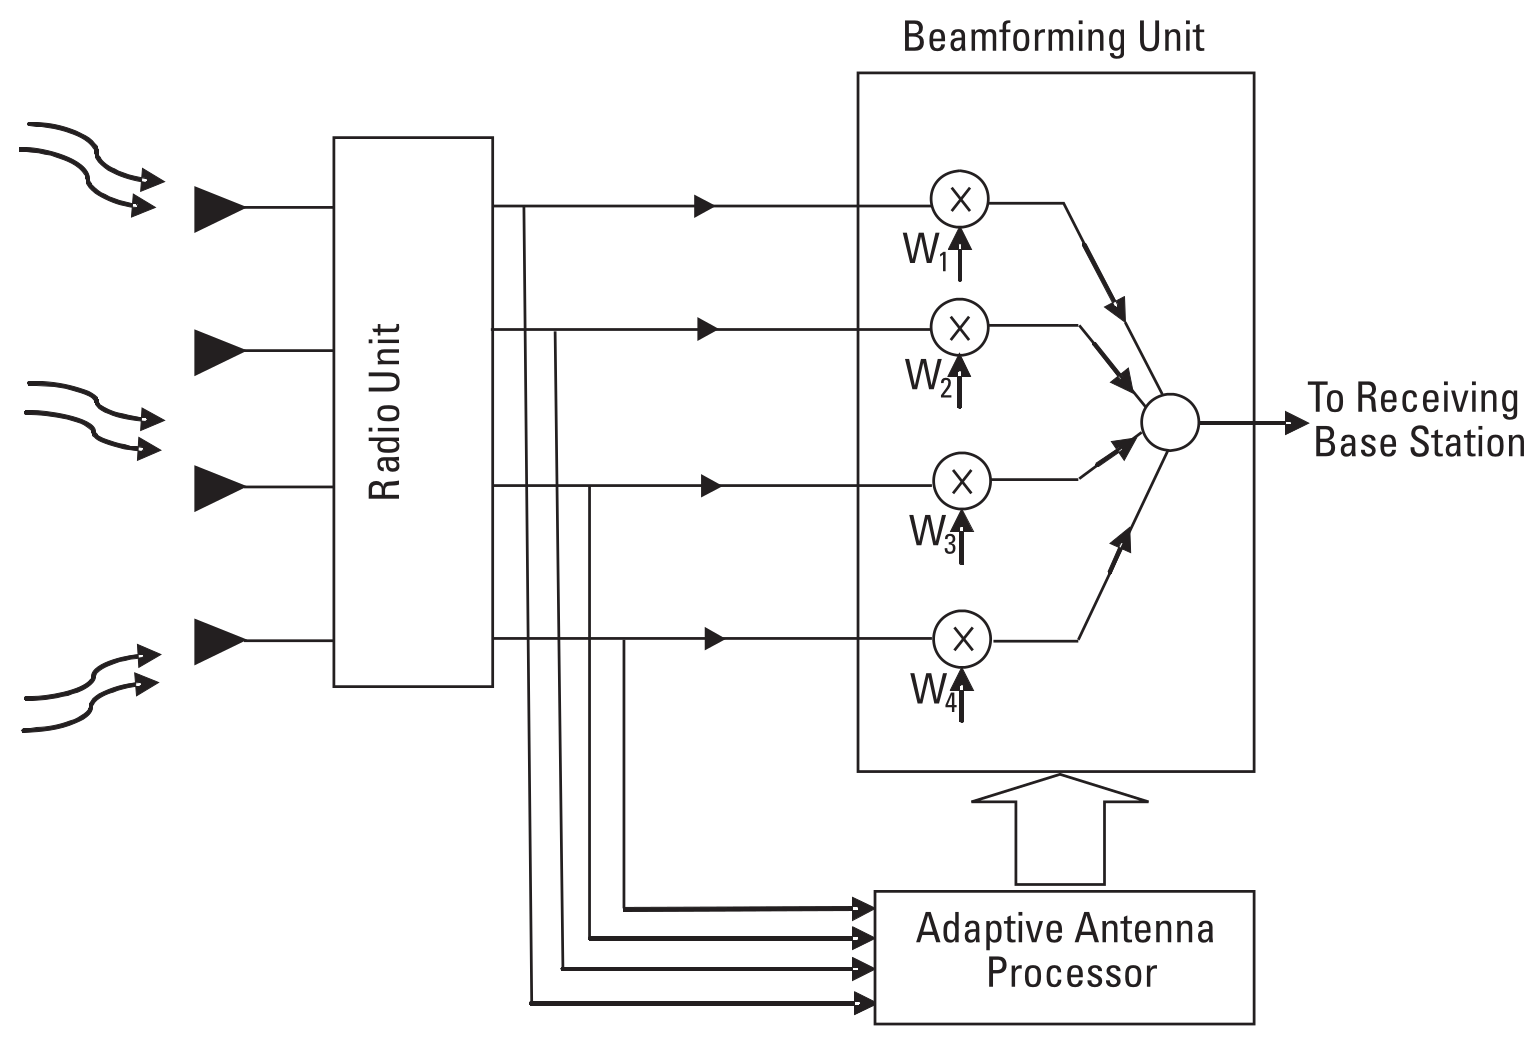
\includegraphics[width=0.7\linewidth]{chapters/figs/fig-1-1}
	\caption{گیرنده آنتن هوشمند}
	\label{fig:1-1}
\end{figure}

\begin{figure}[h]
	\centering
	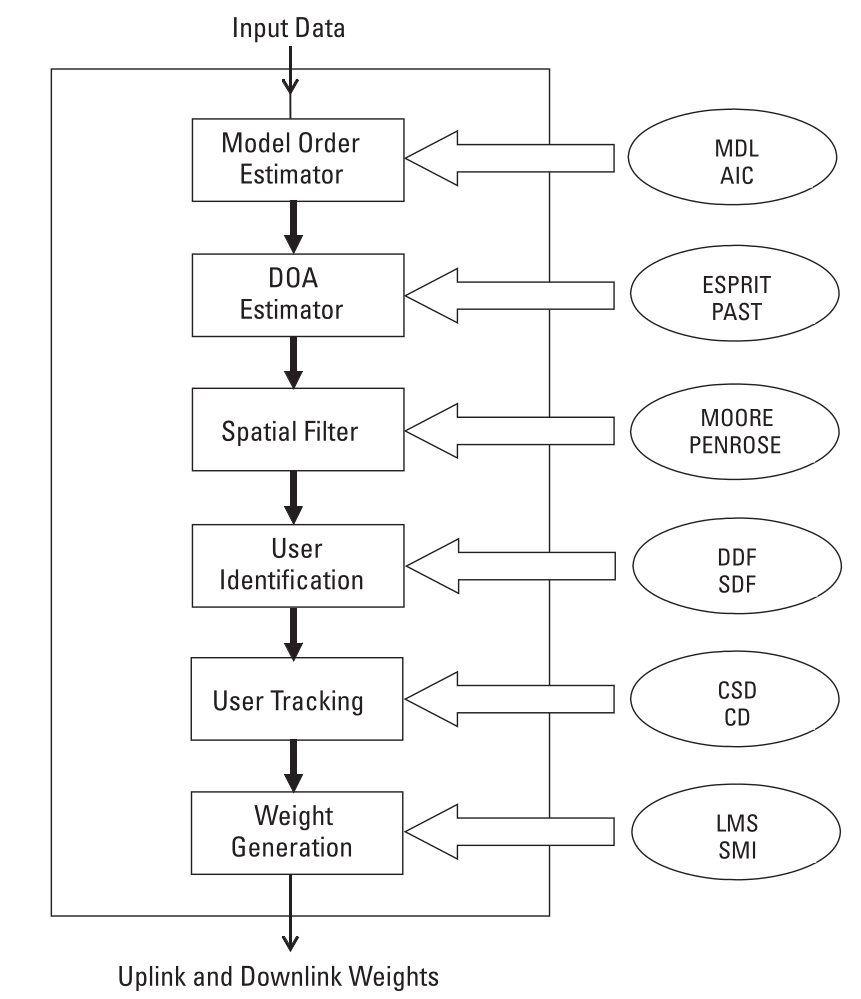
\includegraphics[width=0.7\linewidth]{chapters/figs/fig-1-2}
	\caption{پردازنده تطبیقی آنتن}
	\label{fig:1-2}
\end{figure}




\begin{itemize}
	
	\item \textbf{واحد رادیویی}\LTRfootnote{Radio Unit}:  
	این واحد عمدتاً شامل بخش‌های زیر است:  
	(1) آرایه‌های آنتنی که سیگنال‌های فرکانس رادیویی (\lr{RF}) را از محیط دریافت می‌کنند؛  
	(2) زنجیره‌های پایین‌تبدیل که حامل(های) سیگنال‌های \lr{RF} دریافتی توسط آرایه آنتنی را حذف می‌کنند؛  
	و (3) مبدل‌های آنالوگ به دیجیتال که سیگنال‌های بدون حامل را برای پردازش بیشتر به سیگنال‌های دیجیتال متناظر تبدیل می‌کنند.  
	
	آرایه‌های آنتنی می‌توانند یک‌بعدی، دوبعدی یا حتی سه‌بعدی باشند، بسته به اینکه بخواهیم به چه بعدی از فضا دسترسی داشته باشیم. الگوی تابش آرایه به نوع المان‌ها، موقعیت نسبی آن‌ها و تحریک هر المان (دامنه و فاز) بستگی دارد~\cite{5}.
	
	\item \textbf{واحد پرتودهی}\LTRfootnote{Beamforming Unit}:  
	واحد پرتودهی مسئول تشکیل و هدایت پرتو در جهت مطلوب است. در این بخش، وزن‌دهی به سیگنال‌های دریافتی (یا ارسالی) اعمال می‌شود. به‌طور کلی، سیگنال‌های داده $x_k$ با $k=0,\ldots,M-1$ که توسط یک آرایه با $M$ المان دریافت می‌شوند، مستقیماً در مجموعه‌ای از ضرایب وزن ضرب می‌شوند تا پرتویی در زاویه دلخواه تشکیل شود.  
	
	به بیان دیگر، با ضرب سیگنال‌های داده در مجموعه‌های مناسبی از وزن‌ها می‌توان مجموعه‌ای از پرتوها با زوایای نشانه‌روی دلخواه ایجاد کرد که نتیجه آن یک بیشینه سیگنال در خروجی پرتودهنده خواهد بود. از نظر ریاضی این رابطه به صورت زیر بیان می‌شود:
	\begin{equation}
		y(\theta_i) = \sum_{k=0}^{M-1} w_{k}^i \, x_k
		\label{eq:1-1}
	\end{equation}
	که در آن $y(\theta_i)$ خروجی پرتودهنده، $x_k$ نمونه داده از المان $k$ام آرایه و 
	
	$w_{k}^i$ وزن مربوط به تشکیل یک پرتو یا ایجاد صفر در زاویه $\theta_i$ است. توضیحات بیشتر درباره رابطه \eqref{eq:1-1} در فصل‌های \ref{chap:chapter2} و \ref{chap:chapter3} ارائه خواهد شد.
	
	با انتخاب مقادیر مناسب برای مجموعه وزن‌ها $w_k$ با $k=0,\ldots,M-1$ می‌توان عملیات هدایت پرتو، ایجاد صفر تطبیقی و شکل‌دهی پرتو را پیاده‌سازی کرد. این وزن‌ها که الگوی تابش را تعیین می‌کنند توسط واحد پردازنده تطبیقی آنتن تولید می‌شوند.
	
	\item \textbf{پردازنده تطبیقی آنتن}\LTRfootnote{Adaptive Antenna Processor}:  
	وظیفه این واحد تعیین وزن‌های مختلط برای واحد پرتودهی است. این وزن‌ها معمولاً بر اساس دو نوع معیار اصلی بهینه می‌شوند: بیشینه‌سازی سیگنال داده از منبع مطلوب (مانند روش‌های لوب سوئیچی یا آرایه فازی) یا بیشینه‌سازی نسبت سیگنال به تداخل (\lr{SIR}) از طریق سرکوب سیگنال منابع تداخل (در آرایه تطبیقی).
	
	از نظر تئوری، با $M$ المان آنتنی می‌توان $M-1$ منبع تداخل را حذف کرد، اما در عمل به دلیل انتشار چندمسیری، این تعداد معمولاً کمتر خواهد بود. روش محاسبه وزن‌ها بسته به نوع معیار بهینه‌سازی متفاوت است.
	
	در حالتی که از روش لوب سوئیچی استفاده شود، گیرنده تمام وزن‌های از پیش تعریف‌شده را آزمایش کرده و وزنی را انتخاب می‌کند که قوی‌ترین سیگنال داده دریافتی را ایجاد کند. اما اگر از روش آرایه فازی یا آرایه تطبیقی استفاده شود ــ که شامل هدایت بیشینه بهره به سمت قوی‌ترین مؤلفه سیگنال است ــ ابتدا جهت‌های ورود سیگنال‌ها (\lr{DOA}) تخمین زده می‌شوند و سپس وزن‌ها متناسب با\textit{ زاویه هدایت}\LTRfootnote{Steering angle} مطلوب محاسبه می‌شوند.
	
\end{itemize}
به‌طور کلی، همان‌طور که در شکل \ref{fig:1-2} نشان داده شده است، پردازشگر آنتن تطبیقی\LTRfootnote{Adaptive antenna processor} از چندین فرآیند محاسباتی تشکیل شده است:

\begin{itemize}
	\item \textbf{تخمین‌گر مرتبه مدل\LTRfootnote{Model order estimator}:} از روی داده‌های ورودی $\bm{x}_k$ برای $k = 0, \dots, M-1$ که توسط عناصر آنتن دریافت می‌شوند، تعداد جبهه‌های موج\LTRfootnote{Wavefronts} تابیده بر آرایه با استفاده از الگوریتم‌های تخمین مرتبه مدل، مانند \lr{AIC} یا \lr{MDL} تخمین زده می‌شود که در فصل \ref{chap:4} شرح داده خواهند شد. آگاهی از تعداد سیگنال‌های تابیده بر آرایه برای الگوریتم‌های تخمین جهت ورود\LTRfootnote{Direction of Arrival (DOA)} حیاتی است؛ از این رو، این الگوریتم‌ها پیش از الگوریتم‌های تخمین \lr{DOA} اجرا می‌شوند.
	
	\item \textbf{تخمین‌گر \lr{DOA}:} این بخش، مرحله حیاتی پردازشگر آنتن تطبیقی را تشکیل می‌دهد که در آن از الگوریتم‌هایی مانند \lr{MUSIC} یا \lr{ESPRIT} برای تخمین جهت ورود تمامی سیگنال‌های تابیده بر آرایه استفاده می‌شود. این مرحله، \lr{DOA}های تمامی سیگنال‌های مرتبط با منابع کاربر و سایر منابع تداخل را ارائه می‌دهد. برای سرعت بخشیدن به فرآیند، به‌جای تخمین فضای سیگنال در هر مرحله، از الگوریتم‌های رهگیری زیرفضا\LTRfootnote{Subspace tracking} مانند \lr{dPAST} و \lr{PAST} (رهگیری زیرفضا با تقریب تصویر\LTRfootnote{Projection Approximation Subspace Tracking}) برای رهگیری بازگشتی زیرفضای سیگنال استفاده می‌شود. معمولاً زیرفضای سیگنال به‌کندی با زمان تغییر می‌کند؛ بنابراین رهگیری این تغییرات نسبت به انجام تخمین کامل زیرفضا کارآمدتر است. سپس می‌توان \lr{DOA}ها را با سرعت بیشتری از این زیرفضاها تخمین زد. توصیفات دقیق این الگوریتم‌های \lr{DOA} در فصل‌های \ref{chap:3}، \ref{chap:4} و \ref{chap:5} ارائه شده است.
	
	\item \textbf{فیلتر مکانی\LTRfootnote{Spatial filter}:} پس از به‌دست آمدن \lr{DOA}های تمامی سیگنال‌های تابیده بر آرایه، سیگنال‌ها با بازسازی برای هر یک از \lr{DOA}های تخمین‌زده‌شده، فیلتر می‌شوند. تخمین سیگنال‌ها از روی \lr{DOA}های تخمین‌زده‌شده معمولاً بازسازی سیگنال\LTRfootnote{Signal reconstruction} یا کپی سیگنال\LTRfootnote{Signal copy} نامیده می‌شود. با در اختیار داشتن \lr{DOA}ها، بردارهای هدایت\LTRfootnote{Steering vectors} متناظر $\bm{a}$ و در نهایت ماتریس هدایت\LTRfootnote{Steering matrix} تخمینی $\bm{A}$ تشکیل می‌شوند. سپس سیگنال از رابطه زیر بازسازی می‌شود:
	\begin{equation}
		\bm{S} = \bm{W}\bm{X}
		\label{eq:1-1}
	\end{equation}
	که در آن $\bm{S}$ ماتریس سیگنال‌های تابیده است که از سیگنال‌های آلوده به نویز (یا سیگنال‌های داده) دریافت شده توسط آرایه $\bm{X}$ استخراج شده است، و ماتریس وزن‌دهی $\bm{W}$ به‌عنوان شبه‌معکوس مور-پنروز\LTRfootnote{Moore-Penrose pseudo inverse} ماتریس هدایت آرایه تخمینی $\bm{A}$ انتخاب می‌شود. جزئیات بیشتر در فصل \ref{chap:3} ارائه شده است.
	
	\item \textbf{شناسایی کاربر\LTRfootnote{User identification}:} زمانی که سیگنال‌ها با توجه به \lr{DOA}های متمایزشان از هم جدا شدند، کاربر موردنظر متناظر با این \lr{DOA}ها باید شناسایی شود. با مقایسه میان‌آیندهای\LTRfootnote{Mid-ambles} دریافت شده (توالی‌های آموزشی\LTRfootnote{Training sequences}) با میان‌آیند کاربر موردنظر، تعداد خطاهای بیتی در توالی آموزشی قابل محاسبه است. زمانی که تعداد خطاهای بیتی از یک آستانه کمتر باشد، یک جبهه موجِ تفکیک‌شده‌ی مکانی و در نتیجه \lr{DOA} متناظر با آن به یک کاربر نسبت داده می‌شود. به این ترتیب، نه تنها یک مسیر واحد، بلکه تمام مسیرهای متعلق به کاربر موردنظر شناسایی می‌شوند. سپس \lr{DOA} مربوط به مسیر کاربر با قوی‌ترین توان لحظه‌ای آشکارسازی می‌شود. به‌عنوان آشکارساز توالی آموزشی، تخمین‌گرهای توالی استاندارد مانند بازخورد تصمیم تأخیری\LTRfootnote{Delayed Decision Feedback (DDF)} و بازخورد تصمیم نرم\LTRfootnote{Soft Decision Feedback (SDF)} به کار می‌روند \cite{6}.
	
	\item \textbf{رهگیری کاربر\LTRfootnote{User tracking}:} یک تخمین‌گر تطبیقی با واکنش سریع برای رهگیری تغییرات پارامترهای سیگنال مورد نیاز است. رهگیر نه تنها از مختل شدن شکل‌دهی پرتو\LTRfootnote{Beamforming} توسط تخمین‌های پرت جلوگیری می‌کند، بلکه مانع از تغییرات بیش از حد تخمین‌های \lr{DOA} بین دو بسته‌ی سیگنال متوالی می‌شود. این امر منطقی است، زیرا یک کاربر متحرک در زمان واقعی طی یک فریم مشاهده، جابجایی زیادی ندارد؛ بنابراین تغییرات \lr{DOA} تدریجی است. رویکرد رهگیری کاربر بر پایه فرمول‌بندی بازگشتی برای رهگیری \lr{DOA}ها استوار است که در آن، تغییرات کوچک در تفاضل تخمین‌های ماتریس همبستگی، منجر به تغییرات کوچک در تفاضل ماتریس‌های هدایت می‌شود که \lr{DOA}ها از طریق آن‌ها استخراج می‌شوند. یکی از مشکلاتی که این الگوریتم‌ها ایجاد می‌کنند، مسئله تناظر داده‌ها\LTRfootnote{Data association} است؛ یعنی نسبت دادن تخمین‌های \lr{DOA} در لحظه زمانی قبلی به لحظه زمانی فعلی. برای غلبه بر این مشکل، الگوریتم‌هایی مانند تندترین نزول مقید\LTRfootnote{Constrained Steepest Descent (CSD)}، تندترین نزول\LTRfootnote{Steepest Descent (SD)} و گرادیان مزدوج\LTRfootnote{Conjugate Gradient (CG)} توسعه یافته و به کار گرفته شده‌اند \cite{7, 8}.
	
	\item \textbf{تولید وزن\LTRfootnote{Weight generation}:} \lr{DOA} رهگیری‌شده با قوی‌ترین توان لحظه‌ای انتخاب می‌شود و بدین ترتیب وزن‌های واحد شکل‌دهی پرتو برای تمرکز تطبیقی پرتوها بر روی منبع موردنظر تولید می‌گردند. الگوریتم‌های آنتن تطبیقی مانند کمترین میانگین مربعات\LTRfootnote{Least Mean Square (LMS)} یا معکوس‌سازی ماتریس نمونه\LTRfootnote{Sample Matrix Inversion (SMI)} \cite{9} برای تولید این وزن‌ها استفاده می‌شوند. انتخاب الگوریتم تطبیقی برای استخراج وزن‌های تطبیقی بسیار حائز اهمیت است، زیرا هم سرعت همگرایی و هم پیچیدگی سخت‌افزاری مورد نیاز برای پیاده‌سازی الگوریتم را تعیین می‌کند.
\end{itemize}




\section{نمای کلی کتاب}
\label{sec:1-2}

الگوریتم‌های تخمین \lr{DOA} قلب سیستم‌های آنتن هوشمند\LTRfootnote{Smart antenna systems} را تشکیل می‌دهند. در تمامی حوزه‌ها، مجموعه‌ای از الگوریتم‌های متنوع تخمین \lr{DOA} برای استفاده در سیستم‌های آنتن هوشمند با هدف کاربردهای موقعیت‌یابی\LTRfootnote{Position-location applications} وجود دارند \cite{10}، و موارد بیشتری نیز در حال ظهور هستند \cite{3, 11}. با این حال، چالش طراح، انتخاب الگوریتم مناسب برای تخمین \lr{DOA} است؛ چرا که پیشرفته‌ترین پیاده‌سازی‌های آنتن هوشمند شامل بیشینه‌سازی هم‌زمان سیگنال مفید و حذف (صفر کردن) منابع تداخل است. حتی با وجود واحدهای قدرتمند پردازش سیگنال که امروزه در دسترس هستند، انجام این کار در زمان واقعی\LTRfootnote{Real time} وظیفه‌ای چالش‌برانگیز است. در نتیجه، کارایی و اثربخشی یک الگوریتم در انتخاب آن برای تخمین \lr{DOA} بسیار حیاتی است. به عبارت دیگر، برای طراحانی که از تکنیک آنتن هوشمند استفاده می‌کنند، درک کامل الگوریتم‌های تخمین \lr{DOA} ضروری است.

هدف این کتاب، ارائه مقدمه‌ای بر مفاهیم پایه تخمین \lr{DOA} به همراه مروری بر تکنیک‌های اساسی آن است. علاوه بر این، الگوریتم‌های متعلق به خانواده \lr{ESPRIT}\LTRfootnote{Estimation of Signal Parameters via Rotational Invariance Techniques (ESPRIT)} (تخمین پارامترهای سیگنال از طریق تکنیک‌های ناورایی چرخشی) با جزئیات بیشتری شرح داده خواهند شد. دلیل این امر، سادگی و قابلیت تفکیک‌پذیری بالای \lr{ESPRIT} به‌عنوان یک الگوریتم تخمین \lr{DOA} مبتنی بر زیرفضای سیگنال است که بسیاری از تکنیک‌های پیشرفته امروزی بر پایه آن توسعه یافته‌اند.

در حال حاضر، کتاب‌های تجاری محدودی در دسترس هستند که به صورت سیستماتیک اصول و تکنیک‌های پایه تخمین \lr{DOA} را توصیف کنند. این کتاب قصد دارد با ارائه یک نمای کلی و تحلیل عملکرد الگوریتم‌های پایه \lr{DOA} و مقایسه آن‌ها با یکدیگر، به غنای این پایگاه دانش بیفزاید. به‌طور خاص، مطالعه سیستماتیک، تحلیل عملکرد و مقایسه الگوریتم‌های تخمین \lr{DOA} متعلق به خانواده \lr{ESPRIT} ارائه شده است. به‌طور خلاصه، این کتاب مبانی نظری تکنیک‌های تخمین \lr{DOA} را ترسیم می‌کند تا خواننده ضمن درک مفاهیم پایه، در صورت تمایل بتواند مباحث پیشرفته \lr{DOA} را دنبال کند \cite{10, 11}.

این کتاب برای مبتدیانی همچون دانشجویان تحصیلات تکمیلی، مهندسان یا تنظیم‌کنندگان مقررات دولتی که نیاز به کسب دیدگاهی سریع نسبت به اصول تخمین \lr{DOA} دارند، تدوین شده است. همچنین برای متخصصانی که مایل به بازنگری و یادآوری دانش خود در زمینه مبانی تخمین \lr{DOA} هستند، مناسب است.

\section{نمادگذاری‌ها}
\label{sec:1-3}

در این اثر، بردارها و ماتریس‌ها با حروف ضخیم (\textit{bold})، اعم از حروف کوچک یا بزرگ، نشان داده می‌شوند. بالانویس‌های $(\cdot)^H$ و $(\cdot)^T$ به‌ترتیب بیانگر ترانهاده‌ی مزدوج مختلط\LTRfootnote{Complex conjugate transposition} و ترانهاده‌ی بدون مزدوج مختلط هستند. خط تیره روی متغیر $(\bar{\cdot})$ نشان‌دهنده مزدوج مختلط است. $E\{\cdot\}$ عملگر امید ریاضی\LTRfootnote{Expectation operator} را نشان می‌دهد. $\mathbb{R}^{m \times n}$ به ماتریس اعداد حقیقی با $m$ سطر و $n$ ستون اشاره دارد. $\mathbb{C}^{m \times n}$ به ماتریس اعداد مختلط با $m$ سطر و $n$ ستون اشاره دارد. علامت $\in$ به معنای «متعلق بودن به» است. ماتریس جابجایی $\bm{\Pi}_p$ که به‌کرات مورد استفاده قرار می‌گیرد و ماتریس قطری در پیوست به‌طور خلاصه توضیح داده شده‌اند. همچنین، تعریفی از ضرب کرونکر\LTRfootnote{Kronecker products} در پیوست ارائه شده است.


























